\chapter{Duuuuupa biskupa xddd}


\qs{Convergence of random variables}
{
When dealing witch convergence of sequences of random variables, a new definition of convergence is needed. This is because the usual notion of a limit doesn't apply to random variables in the usual sense. To that end, several notions of convergence are defined:
\begin{itemize}
    \item Weak convergence: $x_n \rightarrow g \leftrightarrow P(\norm{x_n-g} > \epsilon ) \rightarrow 0$
        \item Strong convergence: same as weak convergence, but the convergence rate has to be faster than $\frac{1}{N}$
        \item Mean-square convergence: $E[(X_n-X)^{2}] \rightarrow  0$
\end{itemize}



\nt{The strong convergence condition can be written as $x_n \rightarrow g \leftrightarrow P(\norm{x_n-g} > \epsilon )*N \rightarrow 0$
  }
Both he strong, and mean-square convergence imply weak convergence, but don't imply anything about each other.

Something something strong law of large numbers, weak law of large numbers, Central limit theorem

$\cdots $
}


\qs{Nonparametric estimation of distribution function}
{
 A distribution function is defined as the integral of a probability density function over its whole domain. The simplest way to estimate it non-parametrically, is to sort every available realization of a random variable, and at each such value in the sorted sequence increase the value of the function by 1, and at the end divide the vale of the function by the number of such samples. Formally, it can be written as:
 \begin{equation}
        \hat{F}(x) = \frac{ \#\{x_i\::\:x_n\le x\}}{N}
 \end{equation}
By introducing the indication function defined as follows:
\begin{equation}
    I(x_i) = \begin{cases}
        1 \; \text{as} \; x_i \le x\\
        0 \; \text{as}\;  x_i > x
    \end{cases}
\end{equation}

We can write the estimator in more commonly used form:
\begin{equation}
    \hat{F}(x) = \frac{1}{N}\Sigma^{N}_{i=0} I(x_i)
\end{equation}
The expected value of this estimator is equal to the true distribution:
\begin{equation}
    E\hat{F}(x) = F(x)
\end{equation}
And its variance equals:
\begin{equation}
    \text{Var}\hat{F}(x) = \frac{F(x)(1-F(x))}{N}
\end{equation}

}


\qs{Nonparametric estimation of p.d.f(Kernel)}
{
We can estimate the probability density function in a non parametric way as follows:
\begin{equation}
    \begin{aligned}
        \hat{f}_N(x) &= \frac{\hat{F}_N(x+\frac{h}{2}) - \hat{F}_N(x-\frac{h}{2})  }{h}\\
        \hat{f}_N(x) &= \frac{\#\{x_k\::\: x - \frac{h}{2}\le x_k \le x + \frac{h}{2}\}}{Nh}
    \end{aligned}
\end{equation}
Where $h$ is the size of the bins of the histogram.\\
This method however is very coarse, it will only give an easily interpretable plot for a relatively large number of data.

The basic idea of this approach is to count the number of samples in some local neighbourhood, and use this count to estimate the probability. The logical extension of this approach, would be to create this neighbourhood around each sample. One can generate such local neighbourhoods along with a local probability estimate using so called kernel functions.


\\
\dfn{Kernel function}
{
    An example of a kernel function (Parzen kernel(???)) would be:
    \begin{equation}
        K(v) = \begin{cases}
            1 \text{ as } \norm{v} \le \frac{1}{2}\\
            0 \text{ otherwise}
        \end{cases}
    \end{equation}
    %% plot


\begin{center}
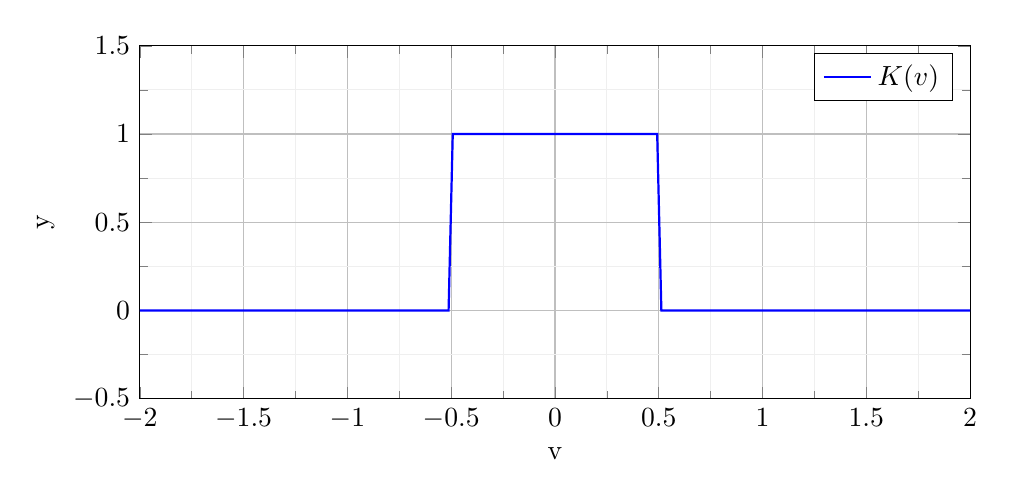
\begin{tikzpicture}
 
\begin{axis}[
    xmin = -2, xmax = 2,
    ymin = -0.5, ymax = 1.5,
    grid = both,
    minor tick num = 1,
    major grid style = {lightgray},
    minor grid style = {lightgray!25},
    width = \textwidth,
    height = 0.5\textwidth,
    xlabel = v,
    ylabel = y]
    \addplot[
        domain = -2:2,
        samples = 200,
        thick,
        blue,
        ] 
        {
        (x > -0.5)*(1)*(x < 0.5)*(1) + 0
        };

    \legend{$K(v)$
           }
\end{axis}
 
\end{tikzpicture}
\end{center}

    When is $K(\frac{x_k-x}{h}) = 1$? This example shows that $K(v)$ plays the role of a selector function, as it will be 1 only when $\norm{x_k-x} \le \frac{1}{2}h$
    \\
    By an appropriate choice of h we can use K(v) to approximate the probability density function.
    \nt{There are many different kinds of kernel functions, the rectangular kernel shown above, the Gaussian kernel, the triangular kernel, etc. \\
    However, in practice all give comparable results, which results in the simplest kernels being most often used. Those being the rectangular kernel - which is the simplest to calculate, but gives non-smooth results - and the Gaussian kernel - which is more difficult to calculate, but gives smoother results}
}


\thm{Kernel probability estimation}
{
    \begin{equation}
        \hat{f}_N(x) = \frac{1}{Nh}\Sigma_{k=1}^{N}K(\frac{x_k-x}{h})
    \end{equation}

    Limit properties ($N \rightarrow \infty$):\\
    How to set $h$ asymptotically?
    \begin{equation}
        \text{If } N \rightarrow \infty
        \begin{cases}
            h(N) \rightarrow 0 \text{ then bias } \hat{f}_n(x) \rightarrow 0\\
            Nh(N) \rightarrow \infty \text{ then } \text{var}\hat{f}(x) \rightarrow 0
        \end{cases}
    \end{equation}

    This means that $h(N) \in \textbf{o}(\frac{1}{N})$ e.g. it has to increase no faster than $\frac{1}{N}$, so for example $h(N) = \frac{1}{\sqrt{N}}$

    \nt{
    In the multidimensional case we get a more restrictive condition on asymptotic behaviour:

 \begin{equation}
        \text{If } N \rightarrow \infty
        \begin{cases}
            h(N) \rightarrow 0 \text{ then bias } \hat{f}_n(x) \rightarrow 0\\
            Nh(N)^{d} \rightarrow \infty \text{ then } \text{var}\hat{f}(x) \rightarrow 0
        \end{cases}
    \end{equation}
Which means that $h(N)$ tends to 0 much more slowly than in the 1D case.
This is known as the \textit{curse of dimensionality}
    }
}
}




\qs{Nonparametric estimation of p.d.f(Othrogonal expansion}
{

    A different approach to nonparametric estimation is based on so called orthogonal basis expansion. To understand what this is, orthogonal functions have to be defined first:
    %%def
    \dfn{Orthogonal functions}
    {
        A set of functions $\{\phi(x)_i\}$ is said to be normal, if the following conditions hold for all of its elements:
        \begin{equation}
            
            \begin{cases}
                \int_D\phi_i^{2}dx = L_i\\
                \int_D\phi_i\phi_j dx = 0
            \end{cases}
        \end{equation}
        If $L_i = 1 \forall i $ then the set can be called orthonormal.
        All orthogonal sets of functions can be made orthonormal through a procedure known as normalization. It is done by dividing each $\phi_i$ by  $\sqrt{L_i}$
    }




  On the domain where these functions are orthogonal, they can be used to define any function in a similar manner to a Taylor series. The only condition for this kind of expansion is that the approximated function is square-integrable(meaning $\int f^{2}(x)dx < \infty$)

  Armed with an orthonormal function basis, and a series of outputs of the function to be estimated, one can estimate the function either as an orthonormal series, or as a rational function of 2 such series.
  \nt{Note that we don't need to know any inputs to the estimated function, we just need realizations of a given random variable to estimate its p.d.f. }

\dfn{An orthogonal series expansion}
{
    We are given(google it) a set of orthogonal functions:
    \begin{equation}
        \{\phi_i(x)\}^{\infty}_{i=1}
    \end{equation}
    A function $f(x)$ can then be written in terms of that basis as follows:
     \begin{equation}
         f(x) = \Sigma_{i=1}^{\infty} a_i\phi_i(x)\;\text{where: }\; a_i = f(x) \dot\phi_i(x)
    \end{equation}

    In this course, we assumed that $f(x)$ is a probability density function. If we assume so, then:
    \begin{equation}
        \begin{aligned}
            a_i &= \int f(x)\phi_i(x)dx &= E\phi_i(x)
        \end{aligned}
    \end{equation}
    Where $E\phi_i(x)$ means the expected value of $\phi_i(x)$.
}

We can't know the true expected value, so instead we can approximate it using a mean:
\begin{equation}
    E\phi(x) \sim \frac{1}{N} \Sigma^{N}_{k=1}\phi_i(x_k) = \hat{a}_i
\end{equation}
This ultimately gives the p.d.f. estimate as:
\begin{equation}
    \hat{f}(x) = \Sigma_{k=0}^{S}\hat{a}_i\phi_i(x)
\end{equation}
Where S is a parameter called scale. As long as it is finite, the above series can only approximate the true function. Due to the assumption of square integrability however, we can be sure that these terms get smaller and smaller very quickly, meaning we can stop the approximation at a relatively small value - say $S = 20$ - and still obtain a satisfactory approximation.\\
To estimate p.d.f. using a ratio, the following relation can be used:
\begin{equation}
    \hat{f}(u) = \frac{\hat{g}(u)}{\hat{f}(u)} = \frac{\Sigma^{S}_{i=1}\hat{b}_i \phi_i(u)}{ \Sigma^{S}_{i=1}\hat{a}_i \phi_i(u)  }
\end{equation}


Where:
\begin{equation}
    \begin{cases}
        \hat{a}_i = \frac{1}{N}\Sigma^{N}_{k=1}\phi_i(u_k)\\
        \hat{b}_i = \frac{1}{N}\Sigma^{N}_{k=1}y_k \phi_i(u_k)
    \end{cases}
\end{equation}






}

\qs{Cross correlation analysis}
{

    Correlation, is defined as normalized covariance of 2 signals:
    \begin{equation}
        \begin{cases}
            \text{cov}(X,Y) = E[(X-EX])(Y-EY)] \text{ - Covariance}\\
            \xi(X,Y) = \frac{\text{cov}(X,Y)}{\sqrt{\text{Var}X\text{Var}Y}} \text{ - Correlation}
        \end{cases}
    \end{equation}
    A random process, is defined as a time dependant random variable:
    \begin{equation}
        X(\omega,t) \text{ - For a specific time instant $t = t_0$, we get a random variable $X_{t_0}(\omega)$, where $\omega$ is some parameter}
    \end{equation}
Assuming $\omega$ to be constant between different time instances, we can define the autocovariance of a stationary random process as follows:

\begin{equation}
    A_X(\tau) = \text{cov}(X_{t_0},X_{t_0+\tau}),\;\text{where $A_X(0) = \sigma^{2}_X$}
\end{equation}
And the autocorrelation as:
\begin{equation}
    r_X(\tau) = \frac{A_X(\tau)}{\sigma^{2}_X}
\end{equation}
Similar definitions follow for the cross-covariance and cross-correlation functions of 2 processes:
\begin{equation}
    \begin{cases}
        W_{X,Y}(\tau) = \text{cov}(X_{t_0},Y_{t_0+\tau})\\
        \cdots 
    \end{cases}
\end{equation}

These definitions can be applied to non-parametric estimation of a system by noticing, that if system's output at time instant k - SISO for clarity - can be written in the following form:
\begin{equation}
    y_k = \Sigma^{\infty}_{i=0}\gamma_iu_{k-i} +z_k
\end{equation}
where:
\begin{itemize}
        \item $u_k$ - i.i.d.
        \item the system is stavle
        \item for simplicity, $Eu_k = 0$
\end{itemize}
\\
We can find the cross correlation function of $u_k$ and  $y_k$ as:
\begin{equation}
    \begin{aligned}
        r_{u,y} &   = E\left\{ u_k \cdot y_{k+\tau}\right\} \\
                &= E\left\{ u_k(\gamma_0 u_{k+\tau} + \gamma_1u_{k+\tau-1}+\dots+z_k)\right\}\\
                &= \sigma^{2}_u \cdot \gamma_\tau
    \end{aligned}
\end{equation}

This finally gives a way to estimate $\gamma_i$ using cross correlation as:
\begin{equation}
    \hat{\gamma}_\tau = \frac{1}{N-\tau} \Sigma_{k=1}^{N-\tau}u_ky_{k+\tau}
\end{equation}


For a Hammerstein system, the cross-correlation of input and output gives:

\begin{equation}
    \begin{aligned}
        r_{u,y}(\tau)&=E\left\{u_k\cdot\left( \gamma_0\mu(u_{k+\tau}) + \gamma_1\mu(u_{k+\tau-1}) + \dots + \gamma_\tau\mu(u_k) + \dots + z_k  \right)\right\}&\mbox{}\\[1.25ex]
        \cdot&=Eu_k\mu(u_k) \cdot \gamma_\tau &\mbox{}\\[1.25ex]
    \end{aligned}
\end{equation}
Which gives:
\begin{equation}
    C_{u,y}(\tau) = r_{u_k,\mu(u_k)}(0)\cdot \gamma_\tau
\end{equation}
\nt{THIS ONLY WORKS FOR WHITE NOISE INPUT!!!!\\
    If the signals $u_k$ were correlated with each
    other then the sum would not simplify to just the single interesting to us term.
    AND THIS DOES NOT WORK FOR WIENER SYSTEM IN GENERAL}

    To make a similar analysis apply to the Wiener system, one has to make the input follow the Gaussian distribution.  This fact was proven by Bussgang, and can be found in "Applied non-parametric regression" written by someone much smarter than us.



}

\qs{Least squares method, offline version(synthesis, propperties)}
{
    
Imagine we have a static system, which is defined with a parameter vector:
\begin{equation}
    a^{*}= \begin{bmatrix}
        a_0^{*} \\
        \vdots\\
        a_s^{*}
    \end{bmatrix}
\end{equation}
Where the $*$ means that the parameters are both true, and unknown.
Imagine then, that the system is supplied with and input vector $x$, and gives a scalar output. So this is a MISO static system.


\dfn{Types of knowledge}
{
    In general, we have 2 kinds of knowledge:
    \begin{itemize}
        \item non-parametric - measurements output pairs: $\{(x_k,y_k)\}_{k=1}^{N}$. A cloud of measured points.
        \item parametric - $y = F^{*}(x,a^{*})+z$, and we know the proverbial shape of the formula $F(x,a)$, but not the exact values of the parameters. We also know, that by using $a^{*}$ as an argument, we'll get the best possible results.
    \end{itemize}
}

\thm{Gauss 1809}
{
    Given that the true process output is modeled as $y = F^{*}(x,a^{*})+z)$, but the shape is given as: $\bar{y} = F(x,a)$. The difference between them should be just the noise, if we managed to match $a = a^{*}$, the expected value of which should be equal to 0.  Gauss proposed a quality term:
  \begin{equation}
      Q(a) = E(y-\bar{y})^{2}
 \end{equation}
 Which is the square of the expected value of the noise, the square makes it always positive.
 The above would require the knowledge of the distribution function of the system, so instead he proposed an estimator:
 \begin{equation}
     \begin{aligned}
         \hat{Q}(a) &= \frac{1}{N} \Sigma_{k=1}^{N}(y_k-\bar{y}_k(a))^{2}\\[1.25ex]
         \hat{Q}(a) &= \frac{1}{N}\Sigma_{k=1}^{N}(F^{*}(x_k,a^{*})+z_k - F^{*}(x_k,a))\\[1.25ex]
     \end{aligned}
 \end{equation}
 This estimator would give the lowest value for $a = a^{*}$, it being $\hat{Q}(a^{*}) = \text{Var}\,z$, which can be written as: $\underset{x}{\arg\min}\,Q(a) = a^{*}$ 

 The condition for which this will converge, is that all measurements $x_k$ are independent. Then, as a consequence of the strong law of large numbers  $\hat{Q} \rightarrow  Q$.


}
For linear system, let:
\begin{equation}
    x = \begin{bmatrix}
        x^{(1)}  \\
        \vdots\\
        x^{(s)}
    \end{bmatrix}
    \;\;
a^{*} = \begin{bmatrix}
        a^{*(1)}  \\
        \vdots\\
        a^{*(s)}
    \end{bmatrix}
\end{equation}
and:
\begin{equation}
    y = x^{T}a^{*} + z = a^{*^{T}}x + z
\end{equation}
Then for each measurement:
\begin{equation}
    y_k = x^{T}_ka^{*} + z_k \text{ for }k\in \mathbb{N}
\end{equation}
So for large k, we'll have a lot of equations. Let us create a dataset of measurements:
\begin{equation}
    Y_N = \begin{bmatrix}
        y_1  \\
        \vdots\\
        y_N
    \end{bmatrix}
    \;\;
    \phi_N = \begin{bmatrix}
        x_1^{(1)} & \hdots & x_1^{S}  \\
        x_1^{(1)} & \hdots & x_2^{S}  \\
              & \vdots &   \\
        x_N^{(1)} & \hdots & x_N^{S}  \\
    \end{bmatrix} = 
    \begin{bmatrix}
        x_1^{T}\\
        \vdots\\
        x_N^{T}
    \end{bmatrix}
\end{equation}
Then we can write the totality of those measurements as a single matrix equation:
\begin{equation}
    Y_k = \phi_N a^{*} + Z_k \text{ with } E(z_k) = 0
\end{equation}
The model however, is defined as:
\begin{equation}
    \bar{Y}_N(a) = \phi_Na
\end{equation}
What we mean to to then, is to minimize the norm of the difference vector:
\begin{equation}
    \begin{aligned}
        \norm{Y_N - Y_N(a)} &= (Y_N - Y_N(a))^{T}(Y_N-Y_N(a))\\[1.25ex]
        \norm{Y_N - Y_N(a)} &= (Y_N - \phi_N(a))^{T}(Y_N-\phi_N(a))\\[1.25ex]
        \norm{Y_N - Y_N(a)} &=Q(a)\\[1.25ex]
        
    \end{aligned}
\end{equation}
After some derivations, we'll obtain:
\begin{equation}
    \nabla_a Q(a) = 0
\end{equation}
The consequence of which is:
\begin{equation}
    \phi_N^{T}\phi_Na = \phi_N^{T}Y_N
\end{equation}
The above is known as the \textbf{normal equation}. This gives us an easy way to calculate the value of a using the pseudo inverse of $\phi_N$:
 \begin{equation}
     \hat{a} = (\phi_N^{T}\phi_N)^{-1}\phi^{T}_N Y_N
\end{equation}


\nt{The same formulation can be used in estimating a dynamic system, by interpreting the multiple inputs of the static system as a history of inputs to the dynamic system}

Something to note is that we only require the system to be linear in its parameters $a^{*}$, the functions which are multiplied by these coefficients are of no consequence. There is a variant of the method where that need not be the case called non-linear least squares, but that wasn't covered during the lecture.\\

Some properties of this method:
\begin{itemize}
        \item As can be seen above, it has a closed form solution which is called the normal equation
        \item It only assumes errors at the output, not the input. This assumption however can be mitigated, but this is not a part of the lecture.
        \item The best, unbiased estimate of the parameter vector is given by the normal equation, assuming that the noise is uncorrelated and has 0 mean.
\end{itemize}


}

\clearpage
\qs{Online least squares}
{

   The normal equation necessitates some difficult matrix calculations, which need to be recalculated with each new data point. This is highly computationally inefficient, and as such an alternative formulation of the least squares method is needed. One can show, that there exists another way to iteratively calculate the least-squares estimator in a 2 step process. This process lacks any similarily difficult calculations, and as such can be even performed in real time as new data arrives. The procedure is as follows:
   \begin{enumerate}
           \item Calculate the so called covariance matrix $P$
           \item Use it to add a correction term to the current estimate of  $\gamma$
           \item 
           
   \end{enumerate}
    \begin{equation}
        \begin{cases}
            P_k = P_{k-1} - \frac{P_{k-1}\phi_k\phi_k^{T}\phi_{k-1}}{1+\phi_k^{T}P_{k-1}\phi_k}\\
            \hat{\gamma}_k = \hat{\gamma}_{k-1} + P_k\phi_k(y_k - \phi_k^{T}\hat{\gamma}_{k-1})
        \end{cases}
    \end{equation}
    Where:
    \begin{itemize}
        \item $\hat{\gamma}_k$ - the k-th estimate of the coefficient vector
        \item  $P_k$ - the covariance matrix, as the approximation converges, its coefficients all go to 0.
        \item  $\phi_k = \begin{bmatrix}
       u_k \\
                  \vdots \\
                  u_{k-n} \\
\end{bmatrix}$ -- vector of last  n inputs, where n is the length of the parameter vector
    \end{itemize}
   This method converges to the exact same value as the least squares method, though its exact value for $k-th$ sample may differ from the offline method. One of the sources of this discrepancy are the initial conditions of the recurrence relation, which may be chosen arbitrarily.\\
Assumptions are the same as for the offline version, though now we can not say that it gives the optimal estimate, despite it converging to the same value. In practice, this loss of optimality is insignificant compared with performance gains.
}


\qs{Instrumental variables}
{
For the purposes of this course, instrumental variables are a tool for removing bias from an estimator of a system, where the output corrupting noise is correlated and not independent. During this course, it was used to remove bias from a least squares estimator of a linear system of the following block structure:
%\begin{figure}[H]
\begin{center}
\begin{tikzpicture}[block/.style = {draw, fill=white, rectangle, minimum height=3em, minimum width=3em},
sum/.style= {draw, fill=white, circle, node distance=1cm},
input/.style = {coordinate},
tmp/.style = {coordinate},
output/.style= {coordinate},
pinstyle/.style = {pin edge={to-,thin,black}},
auto,
node distance = 2cm,
>=latex'
]
    
    
    
    \node [input, name=rinput] (rinput) {};
    \node [tmp, right of=rinput] (ins_line) {};
    \node [block, right of=ins_line] (mu) {Linear Block};
    \node [block, below of=mu] (ins) {LS Model};
    \node [output, right of=ins] (ins_out) {};
    \node [sum, right of=mu,node distance=3cm] (sum1) {$+$};
    \node [block, above of=sum1] (F) {F};
    \node [input, above of=F] (noise_F) {};
    \node [output, right of=sum1] (output2) {};



    \draw [-] (rinput) -- node{$u_k$} (ins_line);
    \draw [->] (ins_line) -- (mu);
    \draw [->] (ins_line) |- (ins);
    \draw [->] (mu) -- node{$v_k$} (sum1);
    \draw [->] (sum1) -- node{$y_k$} (output2);
    \draw [->] (ins) -- node{$\bar{y}_k$} (ins_out);
    \draw [->] (noise_F) -- node{$\epsilon_k$} (F);
    \draw [->] (F) -- node{$z_k$} (sum1);

\end{tikzpicture}
\end{center}

%\end{figure}
\\
Here, the output $y_k = a^{T}y + b^{T}u + z_k$, where $z_k$ is a correlated additive noise, for example of the form:
 \begin{equation}
     z_k = 0.5z_{k-1}+\epsilon_k
\end{equation}

If we apply the least squares method to this system, we're going to obtain biased results. To use instrumental variables to help alleviate this problem, one first constructs an approximate system output $\bar{y}_k$, which is by definition not noise corrupted. Then, one applies a different correction step to remove the correlated noise. This can be done in both an online, and offline fashion.\\
Offline:\\
\textbf{Least squares}:
 \begin{equation}
     \hat{a} = (\phi_N^{T}\phi_N)^{-1}\phi^{T}_N Y_N
\end{equation}

\textbf{Instrumental least squares}:\\

 \begin{equation}
     \hat{a} = (\psi_N^{T}\phi_N)^{-1}\psi^{T}_N Y_N
\end{equation}
Online:
 \textbf{Least squares}:\\
    \begin{equation}
        \begin{cases}
            P_k = P_{k-1} - \frac{P_{k-1}\phi_k\phi_k^{T}\phi_{k-1}}{1+\phi_k^{T}P_{k-1}\phi_k}\\
            \hat{\gamma}_k = \hat{\gamma}_{k-1} + P_k\phi_k(y_k - \phi_k^{T}\hat{\gamma}_{k-1})
        \end{cases}
    \end{equation}
    Where:
    \begin{itemize}
        \item $\hat{\gamma}_k$ - the k-th estimate of the coefficient vector
        \item  $P_k$ - the covariance matrix, as the approximation converges, its coefficients all go to 0.
        \item  $\phi_k = \begin{bmatrix}
       u_k \\
                  \vdots \\
                  u_{k-s \\
                  y_{k-1}\\
              \vdots\\
          y_{k-p}} \\
\end{bmatrix}$ -- vector of last s inputs, and p inputs determining the dynamics of the original system.

    \end{itemize}
\\
\textbf{Instrumental Least Squares}:

    \begin{equation}
        \begin{cases}
            P_k = P_{k-1} - \frac{P_{k-1}\psi_k\phi_k^{T}\phi_{k-1}}{1+\phi_k^{T}P_{k-1}\psi_k}\\
            \hat{\gamma}_k = \hat{\gamma}_{k-1} + P_k\psi_k(y_k - \phi_k^{T}\hat{\gamma}_{k-1})
        \end{cases}
    \end{equation}
    Where:
    \begin{itemize}
        \item $\hat{\gamma}_k$ - the k-th estimate of the coefficient vector
        \item  $P_k$ - the covariance matrix, as the approximation converges, its coefficients all go to 0.
        \item  $\phi_k = \begin{bmatrix}
       u_k \\
                  \vdots \\
                  u_{k-s \\
                  y_{k-1}\\
              \vdots\\
          y_{k-p}} \\
\end{bmatrix}$ -- vector of last s inputs, and p inputs determining the dynamics of the original system.

\item  $\psi_k = \begin{bmatrix}
       u_k \\
                  \vdots \\
                  u_{k-s \\
                      \bar{y}_{k-1}\\
              \vdots\\
          \bar{y}_{k-p}} \\
\end{bmatrix}$ -   -- vector of last s inputs, and p inputs determining the dynamics of the instrumental system.
    \end{itemize}



\\
Both systems are equivalent in the sense that they approach the same solution. The instrumental case can be thought of as a special case of the ordinary least squares, as if the output noise is uncorrelated, both $\psi$ and  $\phi$ will be the same.
\\
\nt{The instrumental system $\bar{y}_k$ is bias free asymptotically, but it may take a vary large amount of data to get the bias of that system lower than the one obtained by ordinary least squares. It may take several orders of magnitude more samples for this unbiased result to converge. }


}

\qs{Hammerstein system identification}
{

    I am tiered, this is very simple so I'll just summarize it without equations. You estimate the first block using either the kernel method, or orthogonal expansion. You obtain the estimate of the non-linearity, which you can then use to estimate the linear part.
    \nt{So you go from $(u_k,y_k)$ to  $(\hat{\mu(u_k)},y_k)$ and perform least squares on the last part. Of note also is that you have to assume some things about the estimate of $\mu$ if you want to estimate it appropriately, for example its value at 0.}

}

\qs{SVD and its applicaiton in system identification}
{
    Singular value decomposition(SVD) is a way to decompose an arbitrary matrix into one rectangular, and 2 square matrices as follows:

\dfn{Eigenvalues}
{
    For a square matrix A, the eigenvalues are defined as:
    \begin{equation}
        \det(A-\lambda I) = 0
    \end{equation}
    If the matrix A is not square, then we can define the eigenvalues using the following observation:
    \begin{equation}
        \rank(A) = \rank(A^{T}) = \rank(A^{T}A) = \rank(AA^{T})
    \end{equation}
    To define them as:
    \begin{equation}
        \det(A^{T}A - \lambda I) = 0
    \end{equation}
    Where $\lambda$ is the eigenvalue of  $A^{T}A$, and $\sqrt{\lambda}$ is the eigenvalue of  $A$. This second eigenvalue is always positive.
}


\thm{SVD}
{
    Any matrix M can be decomposed as follows:
    \begin{equation}
        M_{r\times c} = P_{r\times r} D_{r\times c} Q^{T}_{c\times c}
    \end{equation}
    Where D is a diagonal matrix D looks as follows:
    \begin{equation}
        D = \begin{bmatrix}
            \sigma_1 & & \\
                     & \ddots & \\
                     & & \sigma_r
        \end{bmatrix}
    \end{equation}
    And both P and Q  are unitary matrices - matrices with each of its rows and column having norm equal to 1, and $P^{T}P = I$.
  D is a matrix of the square roots of eigenvalues of  $MM^{T}$ or $M^{T}M$
}
The way this can be used in system identification, is when we have a system that is linear in products of its coefficients - as for example in the case of a Wiener system - Where it can be used to extract the individual coefficients up to a multiplicative constant - not their products - based on the least squares estimate of the products.


Given a system with topology:\\
    \begin{center}
\begin{tikzpicture}[block/.style = {draw, fill=white, rectangle, minimum height=3em, minimum width=3em},
sum/.style= {draw, fill=white, circle, node distance=1cm},
input/.style = {coordinate},
tmp/.style = {coordinate},
output/.style= {coordinate},
pinstyle/.style = {pin edge={to-,thin,black}},
auto,
node distance = 2cm,
>=latex'
]
    \node [input, name=rinput] (rinput) {};
    \node [block, right of=rinput] (controller) {$\mu(\cdot)$};
    \node [block, right of=controller] (mu) {$\{ \gamma_k\}$};
    \node [sum, right of=mu,node distance=2cm] (sum2) {$+$};
    \node [tmp, above = 1cm of sum2](noise);  %
    \node [output, right of=sum2, node distance=2cm] (output) {};
    \draw [->] (rinput) -- node{$u_k$} (controller);
    \draw [->] (controller) -- node{$w_k$} (mu);
    \draw [->] (mu) -- (sum2);
    \draw [->] (sum2) -- node{$v_k$} (output);
    \draw [->] (noise)-- node{$z_k$}(sum2);
\end{tikzpicture}
\end{center}

\\

A linear block of the form:
\begin{equation}
    \begin{aligned}
        v_k &= \gamma_0w_k + \gamma_1w_{k-1} + \dots \gamma_nw_{k-n} + z_k \\
        v_k &= \begin{bmatrix}
            \gamma_0 & \dots  & \gamma_n
        \end{bmatrix} \begin{bmatrix}
            w_k \\  \vdots \\ w_0
        \end{bmatrix} = \gamma^{T} w
        
    \end{aligned}
\end{equation}
And a non-linearity:


\begin{equation}
    \begin{aligned}
        \mu(u) &= c_1f_1(u) + c_2f_2(u) + \dots + c_mf_m(u)\\
        \mu(u) &= \begin{bmatrix}
            c_1 & \dots  & c_m
        \end{bmatrix} \begin{bmatrix}
            f_1(u) \\  \vdots \\ f_m(u)
        \end{bmatrix} = c^{T} f(u)
        
    \end{aligned}
\end{equation}

We can create a matrix:
\begin{equation}
    M = c \gamma^{T}
\end{equation}
If we then perform SVD of this matrix, we will recover both coefficient vectors up to a multiplicative constant:
\begin{equation}
    \text{SVD}(M) = \begin{bmatrix}  c & \vdots  
    \end{bmatrix} \begin{bmatrix}
        \sigma_1 & \dots  \\
        \vdots & \ddots
    \end{bmatrix}
    \begin{bmatrix}
        \gamma   \\
        \dots
    \end{bmatrix}
\end{equation}

Note that all the rows of $M$ are linear combinations of 2 vectors, as such, only one singular value exits.
In practice, we don't actually have $M$ at our disposal, so instead we use its least squares estimate $\hat{M}$





}
